% Options for packages loaded elsewhere
\PassOptionsToPackage{unicode}{hyperref}
\PassOptionsToPackage{hyphens}{url}
%
\documentclass[
  11pt,
]{article}
\usepackage{amsmath,amssymb}
\usepackage[]{mathpazo}
\usepackage{ifxetex,ifluatex}
\ifnum 0\ifxetex 1\fi\ifluatex 1\fi=0 % if pdftex
  \usepackage[T1]{fontenc}
  \usepackage[utf8]{inputenc}
  \usepackage{textcomp} % provide euro and other symbols
\else % if luatex or xetex
  \usepackage{unicode-math}
  \defaultfontfeatures{Scale=MatchLowercase}
  \defaultfontfeatures[\rmfamily]{Ligatures=TeX,Scale=1}
\fi
% Use upquote if available, for straight quotes in verbatim environments
\IfFileExists{upquote.sty}{\usepackage{upquote}}{}
\IfFileExists{microtype.sty}{% use microtype if available
  \usepackage[]{microtype}
  \UseMicrotypeSet[protrusion]{basicmath} % disable protrusion for tt fonts
}{}
\makeatletter
\@ifundefined{KOMAClassName}{% if non-KOMA class
  \IfFileExists{parskip.sty}{%
    \usepackage{parskip}
  }{% else
    \setlength{\parindent}{0pt}
    \setlength{\parskip}{6pt plus 2pt minus 1pt}}
}{% if KOMA class
  \KOMAoptions{parskip=half}}
\makeatother
\usepackage{xcolor}
\IfFileExists{xurl.sty}{\usepackage{xurl}}{} % add URL line breaks if available
\IfFileExists{bookmark.sty}{\usepackage{bookmark}}{\usepackage{hyperref}}
\hypersetup{
  pdftitle={My very own Rmarkdown cheat sheet},
  pdfauthor={RF},
  pdfkeywords={how, to, rmarkdown},
  hidelinks,
  pdfcreator={LaTeX via pandoc}}
\urlstyle{same} % disable monospaced font for URLs
\usepackage[margin = 1in]{geometry}
\usepackage{color}
\usepackage{fancyvrb}
\newcommand{\VerbBar}{|}
\newcommand{\VERB}{\Verb[commandchars=\\\{\}]}
\DefineVerbatimEnvironment{Highlighting}{Verbatim}{commandchars=\\\{\}}
% Add ',fontsize=\small' for more characters per line
\usepackage{framed}
\definecolor{shadecolor}{RGB}{248,248,248}
\newenvironment{Shaded}{\begin{snugshade}}{\end{snugshade}}
\newcommand{\AlertTok}[1]{\textcolor[rgb]{0.94,0.16,0.16}{#1}}
\newcommand{\AnnotationTok}[1]{\textcolor[rgb]{0.56,0.35,0.01}{\textbf{\textit{#1}}}}
\newcommand{\AttributeTok}[1]{\textcolor[rgb]{0.77,0.63,0.00}{#1}}
\newcommand{\BaseNTok}[1]{\textcolor[rgb]{0.00,0.00,0.81}{#1}}
\newcommand{\BuiltInTok}[1]{#1}
\newcommand{\CharTok}[1]{\textcolor[rgb]{0.31,0.60,0.02}{#1}}
\newcommand{\CommentTok}[1]{\textcolor[rgb]{0.56,0.35,0.01}{\textit{#1}}}
\newcommand{\CommentVarTok}[1]{\textcolor[rgb]{0.56,0.35,0.01}{\textbf{\textit{#1}}}}
\newcommand{\ConstantTok}[1]{\textcolor[rgb]{0.00,0.00,0.00}{#1}}
\newcommand{\ControlFlowTok}[1]{\textcolor[rgb]{0.13,0.29,0.53}{\textbf{#1}}}
\newcommand{\DataTypeTok}[1]{\textcolor[rgb]{0.13,0.29,0.53}{#1}}
\newcommand{\DecValTok}[1]{\textcolor[rgb]{0.00,0.00,0.81}{#1}}
\newcommand{\DocumentationTok}[1]{\textcolor[rgb]{0.56,0.35,0.01}{\textbf{\textit{#1}}}}
\newcommand{\ErrorTok}[1]{\textcolor[rgb]{0.64,0.00,0.00}{\textbf{#1}}}
\newcommand{\ExtensionTok}[1]{#1}
\newcommand{\FloatTok}[1]{\textcolor[rgb]{0.00,0.00,0.81}{#1}}
\newcommand{\FunctionTok}[1]{\textcolor[rgb]{0.00,0.00,0.00}{#1}}
\newcommand{\ImportTok}[1]{#1}
\newcommand{\InformationTok}[1]{\textcolor[rgb]{0.56,0.35,0.01}{\textbf{\textit{#1}}}}
\newcommand{\KeywordTok}[1]{\textcolor[rgb]{0.13,0.29,0.53}{\textbf{#1}}}
\newcommand{\NormalTok}[1]{#1}
\newcommand{\OperatorTok}[1]{\textcolor[rgb]{0.81,0.36,0.00}{\textbf{#1}}}
\newcommand{\OtherTok}[1]{\textcolor[rgb]{0.56,0.35,0.01}{#1}}
\newcommand{\PreprocessorTok}[1]{\textcolor[rgb]{0.56,0.35,0.01}{\textit{#1}}}
\newcommand{\RegionMarkerTok}[1]{#1}
\newcommand{\SpecialCharTok}[1]{\textcolor[rgb]{0.00,0.00,0.00}{#1}}
\newcommand{\SpecialStringTok}[1]{\textcolor[rgb]{0.31,0.60,0.02}{#1}}
\newcommand{\StringTok}[1]{\textcolor[rgb]{0.31,0.60,0.02}{#1}}
\newcommand{\VariableTok}[1]{\textcolor[rgb]{0.00,0.00,0.00}{#1}}
\newcommand{\VerbatimStringTok}[1]{\textcolor[rgb]{0.31,0.60,0.02}{#1}}
\newcommand{\WarningTok}[1]{\textcolor[rgb]{0.56,0.35,0.01}{\textbf{\textit{#1}}}}
\usepackage{longtable,booktabs,array}
\usepackage{calc} % for calculating minipage widths
% Correct order of tables after \paragraph or \subparagraph
\usepackage{etoolbox}
\makeatletter
\patchcmd\longtable{\par}{\if@noskipsec\mbox{}\fi\par}{}{}
\makeatother
% Allow footnotes in longtable head/foot
\IfFileExists{footnotehyper.sty}{\usepackage{footnotehyper}}{\usepackage{footnote}}
\makesavenoteenv{longtable}
\usepackage{graphicx}
\makeatletter
\def\maxwidth{\ifdim\Gin@nat@width>\linewidth\linewidth\else\Gin@nat@width\fi}
\def\maxheight{\ifdim\Gin@nat@height>\textheight\textheight\else\Gin@nat@height\fi}
\makeatother
% Scale images if necessary, so that they will not overflow the page
% margins by default, and it is still possible to overwrite the defaults
% using explicit options in \includegraphics[width, height, ...]{}
\setkeys{Gin}{width=\maxwidth,height=\maxheight,keepaspectratio}
% Set default figure placement to htbp
\makeatletter
\def\fps@figure{htbp}
\makeatother
\setlength{\emergencystretch}{3em} % prevent overfull lines
\providecommand{\tightlist}{%
  \setlength{\itemsep}{0pt}\setlength{\parskip}{0pt}}
\setcounter{secnumdepth}{5}

% for adjustwidth environment
\usepackage[strict]{changepage}

% for formal definitions
\usepackage{framed}
% environment derived from framed.sty: see leftbar environment definition
\definecolor{formalshade}{rgb}{0.95,0.95,1}

\newenvironment{formal}{%
  \def\FrameCommand{%
    \hspace{1pt}%
    {\color{gray}\vrule width 2pt}%
    {\color{white}\vrule width 4pt}%
    \colorbox{white}%
  }%
  \MakeFramed{\advance\hsize-\width\FrameRestore}%
  \noindent\hspace{-4.55pt}% disable indenting first paragraph
  \begin{adjustwidth}{}{7pt}%
  \vspace{2pt}\vspace{2pt}%
}
{%
  \vspace{2pt}\end{adjustwidth}\endMakeFramed%
}
\usepackage{setspace}\doublespacing
\usepackage[left]{lineno}
\usepackage{dcolumn}
\usepackage{caption}
\usepackage{float}
\usepackage{afterpage}
\usepackage{amsmath}
\ifluatex
  \usepackage{selnolig}  % disable illegal ligatures
\fi
\newlength{\cslhangindent}
\setlength{\cslhangindent}{1.5em}
\newlength{\csllabelwidth}
\setlength{\csllabelwidth}{3em}
\newenvironment{CSLReferences}[2] % #1 hanging-ident, #2 entry spacing
 {% don't indent paragraphs
  \setlength{\parindent}{0pt}
  % turn on hanging indent if param 1 is 1
  \ifodd #1 \everypar{\setlength{\hangindent}{\cslhangindent}}\ignorespaces\fi
  % set entry spacing
  \ifnum #2 > 0
  \setlength{\parskip}{#2\baselineskip}
  \fi
 }%
 {}
\usepackage{calc}
\newcommand{\CSLBlock}[1]{#1\hfill\break}
\newcommand{\CSLLeftMargin}[1]{\parbox[t]{\csllabelwidth}{#1}}
\newcommand{\CSLRightInline}[1]{\parbox[t]{\linewidth - \csllabelwidth}{#1}\break}
\newcommand{\CSLIndent}[1]{\hspace{\cslhangindent}#1}

\title{\textbf{My very own Rmarkdown cheat sheet}}
\author{RF}
\date{October 06, 2021}

\begin{document}
\maketitle
\begin{abstract}
Place holder
\end{abstract}

{
\setcounter{tocdepth}{2}
\tableofcontents
}
\hypertarget{introduction}{%
\section{Introduction}\label{introduction}}

Here live several examples on how to write stuff in Rmarkdown, with no apparent organisation. They are here to help you write a paper using only Rmarkdown and discard every other software away.

\hypertarget{smaller-headlines}{%
\subsection{Smaller headlines}\label{smaller-headlines}}

There are 4 in total, just add more ``\#''

\hypertarget{three-dash-headline}{%
\subsubsection{Three dash headline}\label{three-dash-headline}}

\hypertarget{the-smallest-headline}{%
\paragraph{The smallest headline}\label{the-smallest-headline}}

\hypertarget{specific-text}{%
\section{Specific text}\label{specific-text}}

Microsoft uses buttons, LateX uses functions and Rmarkdown uses symbol shortcut to write specific text:

\emph{I write in italic using} * around the expression (\_ works too)

\textbf{Bold is a possibility too using} **

\texttt{In\ text\ code} such as a \texttt{variable} or a \texttt{function()} is done using `

Subscripts uses \textasciitilde{} and superscripts \^{}, e.g.~H\textasciitilde3\textasciitilde PO\^{}2+\^{} renders H\textsubscript{3}PO\textsuperscript{2+}

And when you want to use any of these symbols verbatim, one needs to add ``\textbackslash{}'' in front

\#, *, `

\hypertarget{highlighting}{%
\subsection{Highlighting}\label{highlighting}}

\begin{quote}
write block quotes using \textgreater{}
\end{quote}

\begin{quote}
however the style appears only in HTML
\end{quote}

There is a workaround using a LateX function:

\begin{formal}
  quote in a pdf
\end{formal}

But you need an associated .tex file which is then given to the YAML

\hypertarget{list-of-items}{%
\subsection{List of items}\label{list-of-items}}

\begin{enumerate}
\def\labelenumi{\arabic{enumi}.}
\tightlist
\item
  one (done using 1.)
\end{enumerate}

\begin{itemize}
\tightlist
\item
  more numbers
\end{itemize}

\begin{enumerate}
\def\labelenumi{\arabic{enumi}.}
\setcounter{enumi}{1}
\tightlist
\item
  two
\end{enumerate}

\begin{itemize}
\item
  not marked using *
\item
  more not marked

  \begin{itemize}
  \item
    nested adding +

    \begin{itemize}
    \tightlist
    \item
      doubling down
    \end{itemize}
  \end{itemize}
\end{itemize}

\hypertarget{others}{%
\subsection{Others}\label{others}}

Rmarkdown can also handle LateX functions such as ``\textbackslash newpage''

\newpage

\hypertarget{math-symbols}{%
\section{Math symbols}\label{math-symbols}}

Mathematics are done using the \$ symbol around the expression. It can be used in line \(X = Y + 1\) or separate and centered using \$\$

\[\alpha = e{^\beta}\]

Specific letters such as \(\alpha\) (written \$\textbackslash alpha\$) must be written in the math environment. The syntax is the same as LateX and can be found on \url{https://www.overleaf.com/learn/latex/List_of_Greek_letters_and_math_symbols}

\hypertarget{citations}{%
\section{Citations}\label{citations}}

Citation are handled using a .bib file, generated by your favorite reference manager (Rmarkdown not doing yet unfortunately)
Add the file path to the YAML at the head of the document (bibliography: myLibrary.bib)

In text citations are done using @ and using the unique code linking to your reference. In my case it looks like ``firstAuthor\_firstWord\_year'' but it is user dependent.

(\protect\hyperlink{ref-andersen_fish_2019}{Andersen 2019}) = {[}@andersen\_fish\_2019{]}

(\protect\hyperlink{ref-andersen_fish_2019}{Andersen 2019}; \protect\hyperlink{ref-blanchard_evaluating_2014}{Blanchard et al. 2014}) = {[}@andersen\_fish\_2019; @blanchard\_evaluating\_2014{]}

\protect\hyperlink{ref-blanchard_evaluating_2014}{Blanchard et al.} (\protect\hyperlink{ref-blanchard_evaluating_2014}{2014}) = @blanchard\_evaluating\_2014

(See \protect\hyperlink{ref-andersen_fish_2019}{Andersen 2019} for details.) = {[}See @andersen\_fish\_2019 for details.{]}

The style of the citations is often journal specific. Fortunately, journals provide .csl files of their own styling, which can be found on \url{https://www.zotero.org/styles}. Dowload the file and give the path to Rmarkdown in the YAML using ``csl: myStyle.csl''

References will be added at the end of the document. Just add a ``\#References'' at the end.

\hypertarget{inserting-code-blocks}{%
\section{Inserting code blocks}\label{inserting-code-blocks}}

Ctrl + Alt + i is the shortcut to insert a code chunk. Useful options are

echo: if TRUE, display code chunk

eval: if TRUE, run the chunk

include: if TRUE, include chunk in doc

message: if TRUE, display code messages

warning: if TRUE, display code warnings

\hypertarget{figures}{%
\section{Figures}\label{figures}}

Figures are added using ! {[}caption{]} (filePath.jpg)

\begin{figure}
\centering

\includegraphics{George.jpg}
\caption{Caption about George}
\end{figure}

For more control over the figure, one can use \texttt{knitr::include\_graphics()}

\newpage

\hypertarget{tables}{%
\section{Tables}\label{tables}}

Tables such as data frame are easily displayed using \texttt{knitr::kable()}

\begin{Shaded}
\begin{Highlighting}[]
\NormalTok{knitr}\SpecialCharTok{::}\FunctionTok{kable}\NormalTok{(}\FunctionTok{head}\NormalTok{(mtcars))}
\end{Highlighting}
\end{Shaded}

\begin{tabular}{l|r|r|r|r|r|r|r|r|r|r|r}
\hline
  & mpg & cyl & disp & hp & drat & wt & qsec & vs & am & gear & carb\\
\hline
Mazda RX4 & 21.0 & 6 & 160 & 110 & 3.90 & 2.620 & 16.46 & 0 & 1 & 4 & 4\\
\hline
Mazda RX4 Wag & 21.0 & 6 & 160 & 110 & 3.90 & 2.875 & 17.02 & 0 & 1 & 4 & 4\\
\hline
Datsun 710 & 22.8 & 4 & 108 & 93 & 3.85 & 2.320 & 18.61 & 1 & 1 & 4 & 1\\
\hline
Hornet 4 Drive & 21.4 & 6 & 258 & 110 & 3.08 & 3.215 & 19.44 & 1 & 0 & 3 & 1\\
\hline
Hornet Sportabout & 18.7 & 8 & 360 & 175 & 3.15 & 3.440 & 17.02 & 0 & 0 & 3 & 2\\
\hline
Valiant & 18.1 & 6 & 225 & 105 & 2.76 & 3.460 & 20.22 & 1 & 0 & 3 & 1\\
\hline
\end{tabular}

It's so simple that it's easier to create a data frame first to make a table, than to make a table directly.

\newpage

\begin{Shaded}
\begin{Highlighting}[]
\NormalTok{param\_description }\OtherTok{\textless{}{-}} \FunctionTok{data.frame}\NormalTok{(}\StringTok{"parameter"} \OtherTok{=} \FunctionTok{c}\NormalTok{(}\StringTok{"w\_inf"}\NormalTok{,}\StringTok{"w\_mat"}\NormalTok{,}\StringTok{"beta"}\NormalTok{),}
                               \StringTok{"description"} \OtherTok{=} \FunctionTok{c}\NormalTok{(}\StringTok{"asymptotic weigth"}\NormalTok{,}
                                                 \StringTok{"maturation weight"}\NormalTok{,}
                                                 \StringTok{"preferred predator/prey mass ratio"}\NormalTok{)}
\NormalTok{)}
\end{Highlighting}
\end{Shaded}

\begin{Shaded}
\begin{Highlighting}[]
\NormalTok{knitr}\SpecialCharTok{::}\FunctionTok{kable}\NormalTok{(param\_description, }\AttributeTok{caption =} \StringTok{"parameters\textquotesingle{} description"}\NormalTok{)}
\end{Highlighting}
\end{Shaded}

\begin{table}

\caption{\label{tab:params}parameters' description}
\centering
\begin{tabular}[t]{l|l}
\hline
parameter & description\\
\hline
w\_inf & asymptotic weigth\\
\hline
w\_mat & maturation weight\\
\hline
beta & preferred predator/prey mass ratio\\
\hline
\end{tabular}
\end{table}

\newpage

\hypertarget{the-neat-stuff}{%
\section{The neat stuff}\label{the-neat-stuff}}

\hypertarget{auto-numbering-and-cross-referencing}{%
\subsection{Auto-numbering and cross-referencing}\label{auto-numbering-and-cross-referencing}}

This is done using the R package \texttt{bookdown}.

\begin{Shaded}
\begin{Highlighting}[]
\FunctionTok{plot}\NormalTok{(mtcars}\SpecialCharTok{$}\NormalTok{mpg,mtcars}\SpecialCharTok{$}\NormalTok{cyl)}
\end{Highlighting}
\end{Shaded}

\begin{figure}
\centering
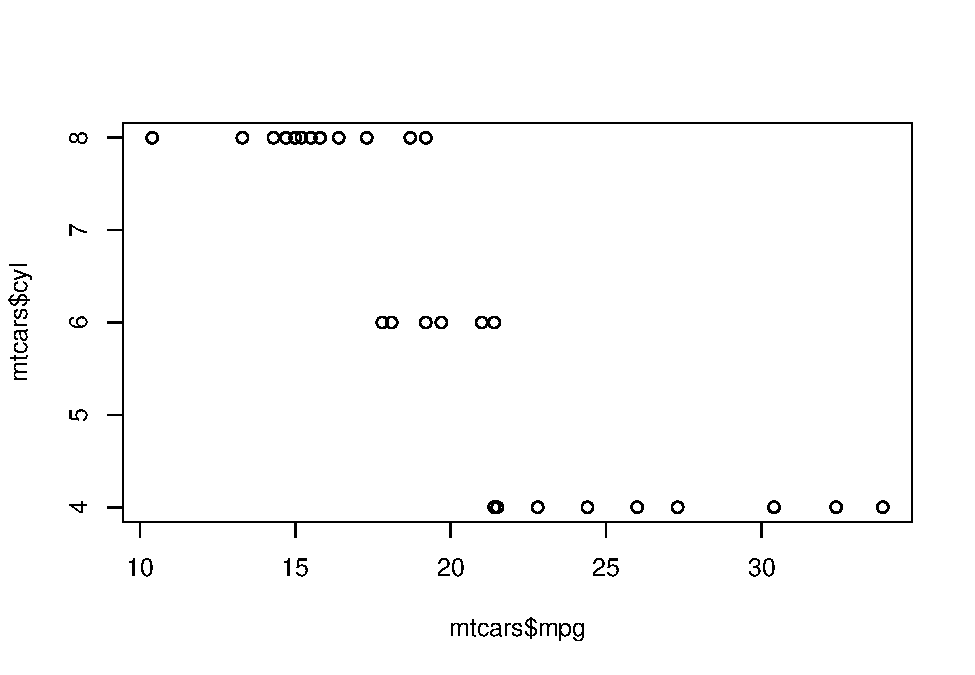
\includegraphics{syntax_files/figure-latex/cars-1.pdf}
\caption{\label{fig:cars}a plot about cars' cylinders}
\end{figure}

Figure \ref{fig:cars} is rad. Table \ref{tab:params} is not bad either.

This reference is done automatically using \textbackslash{} ~@ ref(label), where label is the name of the code-chunk referenced with its float identity, i.e the previous figure's label is \texttt{fig:cars} and the table's label is \texttt{tab:params}

\hypertarget{using-variables-in-text}{%
\subsection{Using variables in text}\label{using-variables-in-text}}

\begin{Shaded}
\begin{Highlighting}[]
\FunctionTok{head}\NormalTok{(mtcars)}
\end{Highlighting}
\end{Shaded}

\begin{verbatim}
##                    mpg cyl disp  hp drat    wt  qsec vs am gear carb
## Mazda RX4         21.0   6  160 110 3.90 2.620 16.46  0  1    4    4
## Mazda RX4 Wag     21.0   6  160 110 3.90 2.875 17.02  0  1    4    4
## Datsun 710        22.8   4  108  93 3.85 2.320 18.61  1  1    4    1
## Hornet 4 Drive    21.4   6  258 110 3.08 3.215 19.44  1  0    3    1
## Hornet Sportabout 18.7   8  360 175 3.15 3.440 17.02  0  0    3    2
## Valiant           18.1   6  225 105 2.76 3.460 20.22  1  0    3    1
\end{verbatim}

The number of cylinders of Mazda RX4 is 6. The previous sentence verbatim is actually:

The number of cylinders of ``r rownames(mtcars){[}1{]}'' is ``r mtcars{[}1,2{]}'' (just need to replace " with ')

\hypertarget{remember-to-checkout-the-yaml}{%
\subsection{Remember to checkout the YAML}\label{remember-to-checkout-the-yaml}}

other stuff?

\hypertarget{cheat-sheets}{%
\section{Cheat sheets}\label{cheat-sheets}}

\url{https://www.markdownguide.org/cheat-sheet}

\url{https://bookdown.org/yihui/rmarkdown-cookbook/basics.html}

\hypertarget{references}{%
\section*{References}\label{references}}
\addcontentsline{toc}{section}{References}

\hypertarget{refs}{}
\begin{CSLReferences}{1}{0}
\leavevmode\hypertarget{ref-andersen_fish_2019}{}%
Andersen, Ken H. 2019. \emph{Fish {Ecology}, {Evolution}, and {Exploitation A New Theoretical Synthesis}}. {Princeton University Press}.

\leavevmode\hypertarget{ref-blanchard_evaluating_2014}{}%
Blanchard, Julia L., Ken H. Andersen, Finlay Scott, Niels T. Hintzen, Gerjan Piet, and Simon Jennings. 2014. {``Evaluating Targets and Trade-Offs Among Fisheries and Conservation Objectives Using a Multispecies Size Spectrum Model.''} Edited by Andre Punt. \emph{Journal of Applied Ecology} 51 (3): 612--22. \url{https://doi.org/10.1111/1365-2664.12238}.

\end{CSLReferences}

\end{document}
